\documentclass[tikz]{standalone}
\usepackage{pgfplots}
\pgfplotsset{compat=1.15}
\usepackage{mathrsfs}
\usetikzlibrary{arrows,calc}
\usepackage{tkz-euclide}

\pagestyle{empty}

\definecolor{AngleClr}{rgb}{0,0.39215686274509803,0}
\definecolor{ShapeClr}{rgb}{0.6,0.2,0}

\begin{document}

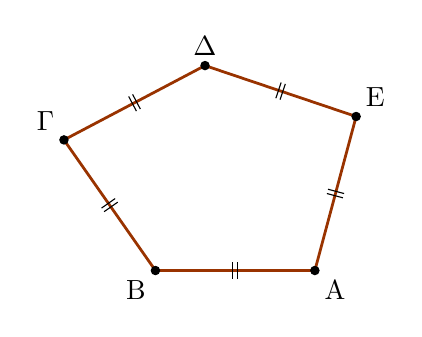
\begin{tikzpicture}[scale=.75]
\tkzSetUpLine[line width=1pt,color=black]
\tkzSetUpPoint[fill=black]

\tkzDefPoints{0/0/P5,2.7/0/P1}

\tkzDefShiftPoint[P5](125:2.7){P4}
\tkzDefShiftPoint[P1](75:2.7){P2}
\tkzInterCC[R](P2,2.7)(P4,2.7) \tkzGetPoints{b}{P3}

\tkzFillPolygon[fill=white](P1,P2,P3,P4,P5)

\tkzDrawPolygon[color=ShapeClr](P1,P2,P3,P4,P5)
\tkzDrawPoints[size=3](P1,P2,P3,P4,P5)
\tkzLabelPoint[below right](P1){$\rm A$}
\tkzLabelPoint[above right](P2){$\rm E$}
\tkzLabelPoint[above](P3){$\rm \Delta$}
\tkzLabelPoint[above left](P4){$\rm \Gamma$}
\tkzLabelPoint[below left](P5){$\rm B$}

\tkzMarkSegments[mark=||,size=3](P1,P2 P2,P3 P3,P4 P4,P5 P5,P1)

\end{tikzpicture}

\end{document}
